\chapter{Sum-of-Squares Clustering}
\label{cha:sum-squar-clust}

\textit{This chapter is largely based on the following paper:}
\vspace{0.5em}

\noindent
\bibentry{kettleborough13sumsquares}\\

% \begin{itemize}
% \item 

%   % George Kettleborough and V.J. Rayward-Smith. Optimising sum-of-squares
%   % measures for clustering multisets over a metric space.
%   % \textit{Discrete Applied Mathematics}, 2013.
% \end{itemize}

\vspace{1em}

\textit{\sffamily My contributions include: the examples showing that
  equations~(\ref{eq:cd-sep-eq}) and (\ref{eq:as-cd-eq}) do not hold for all
  metrics, the example to show that linear separability does not hold for
  all-squares clustering in Section~\ref{sec:linear-separability}, the proof
  for Lemma~\ref{lem:eq-dis}, the proof of
  Theorems~\ref{thm:np-complete-3-val}, \ref{thm:asc-np-complete-n-val} and
  \ref{thm:cdc-np-complete-n-val}, the examples of using the assignment metric
  in Section~\ref{sec:lifting-metric-space}, and the examples leading to
  Theorem~\ref{thm:worst-case}.  I was also responsible for preparation of the
  published manuscript and implementation of the assignment metric for
  testing.  }
\newpage

\section{Introduction}
\label{sec:ss-introduction}

\subsection{Summary}
\label{sec:summary-sum-squar}

\textsc{In this chapter} we examine two sum-of-squares criteria for clustering
in a metric space and compare their performance.  It has recently been shown
that partitional clustering under the centroid-distance criterion is an
NP-hard problem in Euclidean space.  We show that the associated decision
problem is NP-complete even in a highly constrained 2-valued metric space, as
well as general $p$-valued metric spaces.  We also show that the problem is
NP-complete under the related all-squares criterion both in Euclidean space
and for a $p$-valued metric.  We propose a new metric for comparing clustering
called the assignment metric which allows us to use information about the
underlying metric space of a clustering to help distinguish different
clustering solutions.  Using this metric we finally show that optimal
clustering solutions under our two different sum-of-squares criteria can be as
different as any two solutions can possibly be.

\subsection{Multiset datasets}
\label{sec:datasets}

The first stage of clustering is to build a dataset in which clusters are to
be found.  These data are often sampled from some set, $M$.  If the objects in
$M$ have a metric, $d$, defined on them then we say that $(M,d)$ is a metric
space.  The same metric is, of course, then defined for any elements sampled
from $M$, so given a dataset, $\dset \subseteq M$, $(\dset,d)$ is itself a
metric space.

However, there is usually no restriction on how many times an element from $M$
may be sampled so, contrary to the name, a dataset is not usually a set, but
is often a multiset.  A multiset can be considered a generalisation of a fuzzy
set, that is an ordered pair $(\dset,\mu_{\dset})$ where $\dset$ is the
\textit{underlying set} and is the \textit{membership function} but with
$\mu_{\dset} \colon \dset \to \mathbb{R}^+$.  For some element $x \in \dset$
$\mu_{\dset}(x) = n$ means that $n$ copies $x$ appear in $(\dset,\mu_{\dset})$
(note that $x \in \dset$ is ordinary set notation).

\subsection{Multiset clusterings}
\label{sec:multiset-clusterings}

A clustering is usually considered to be a set of subsets of the dataset but
if the dataset is a multiset then the clusters must also be multisets.  A
$k$-clustering of $(\dset,\mu_{\dset})$ is therefore $\clus =
\{(C_{1},\mu_{1}),(C_{2},\mu_{2}),\dotsc,(C_{k},\mu_{k})\}$ where $\mu_i$ is
the membership function for cluster $C_i$.  For any such clustering we have
that $C_{1} \cup C_{2} \cup \dotsb \cup C_{k} = \dset$ and for all $x \in
\dset$, $\sum_{i=1}^{k} \mu_{i}(x) = \mu_{\dset}(x)$.  We will see later that
there are some surprising differences between normal clusterings and multiset
clusterings (see Theorem~\ref{thm:2-met-multiset-np-complete}).

\section{Clustering criteria}
\label{sec:clustering-criteria}

\textsc{As discussed in} Section~\ref{sec:criteria}, the problem of clustering
is finding a solution where the clusters are both homogeneous, meaning
elements belonging to the same cluster are similar, and well-separated,
meaning elements belonging to different clusters are dissimilar.  We have seen
that there are a large number of possible $k$-clustering solutions for any
given dataset and many criteria for judging the homogeneity, separation or
both of a given solution.

In this chapter we will look at the two sum-of-squares criteria which judge
the suitability of a $k$-clustering based on both homogeneity and separation.
We derived the two criteria, called centroid-distance and all-squares, from
the scatter matrix in Section~\ref{sec:scatter-matrix-based}.  We state them
again here defined as cost functions along with definitions of their
corresponding optimal partitions.

The \textit{all-squares cost} of a clustering is defined as:
\begin{equation}
  \label{eq:ASC}
  cost_{as}(\clus) = \sum_{i=1}^{k} \sum_{x,y \in C_i} \mu_i(x) \mu_i(y) d^2(x,y).
\end{equation}

\begin{dfn}
  A multiset $k$-clustering which minimises the all-squares cost for a
  particular $\dset$ is called an all-squares optimal $k$-clustering of
  $\dset$.
\end{dfn}

The \textit{centroid-distance cost} is defined as:
\begin{equation}
  \label{eq:CDC}
  cost_{cd}(\clus) = \sum_{i=1}^{k} \sum_{x \in C_i} \mu_i(x) d^2(x,c_i),
\end{equation}
where $c_i$ is the centroid of $C_i$ and is defined as
\begin{equation*}
  c_i = \argmin_{c \in M} \sum_{x \in C_i} \mu_i(x) d^2(x,c).
\end{equation*}
Calculation of the centroid depends on the metric; for example, with the
Euclidean metric the centroid is the mean, with the overlap metric it is the
mode and with the heterogeneous Euclidean-overlap metric (HEOM, as defined in
Section~\ref{sec:mixed-data-metrics}) it is a mixture of means and modes.

\begin{dfn}
  A multiset $k$-clustering which minimises the centroid-distance cost for a
  particular $\dset$ is called a centroid-distance optimal $k$-clustering of
  $\dset$.
\end{dfn}

Centroid-distance cost is a well known criterion which is often called
sum-of-squares without qualification in the literature (see, for example,
\citep{aloise09,merle1999interior,spath80,jain-1999,hansen1997mathprog}).  We
believe that both of the criteria which we have stated can equally well be
called sum-of-squares criteria, so we qualify them as all-squares and
centroid-distance.

If $d$ is the Euclidean metric, centroid-distance is also equivalent to a
criterion for separation, although it is not immediately obvious why.  It is
due to the parallel axis theorem, or Huygens-Steiner theorem, which we saw in
Section~\ref{sec:scatter-matrix-based}.  The theorem states that when
$(M,d_E)$ is the Euclidean space with the Euclidean metric
\begin{equation}
  \label{eq:huygens}
  \sum_{x \in A} \mu_A(x) d_E^2(x,s)
  = \sum_{x \in A} \mu_A(x) d_E^2(a,s)
  + \sum_{x \in A} \mu_A(x) d_E^2(x,a)
\end{equation}
for each $A \subseteq M$, where $a \in M$ is the centroid of $A$, and $s \in
M$ \citep{spath80}.  By summing over each clustering, $C_1,\dotsc,C_k$ in some
clustering of $\dset$ we obtain the equation:
\begin{equation}
  \label{eq:cd-sep-eq}
  \sum_{x \in \dset} \mu_{\dset}(x) d_E^2(x,s)
  = \sum_{i=1}^{k} \sum_{x \in C_i} \mu_i(x) d_E^2(c_i,s)
  + \sum_{i=1}^{k} \sum_{x \in C_i} \mu_i(x) d_E^2(x,c_i).
\end{equation}
The left-hand side is a constant for any $s$ and $\dset$ and the second term
on the right-hand side is the centroid-distance cost.  Therefore, minimising
the centroid-distance cost is equivalent to maximising squared-separation
\begin{equation*}
  sep(\clus) = \sum_{i=1}^{k} \sum_{x \in C_i} \mu_i(x) d_E^2(c_i,s).
\end{equation*}
For convenience, $s$ is usually taken to be the centroid of $\dset$.

We can also use equation~\eqref{eq:huygens} to show an alternative formula for
centroid-distance cost.  We substitute some $y \in C_i$ for $s$ in
\eqref{eq:huygens} and sum over all $y \in C_i$, multiplying each term by
$\mu_i(y)$:
\begin{eqnarray*}
  \sum_{y \in C_i} \sum_{x \in C_i} \mu_i(x) \mu_i(y) d_E^2(x,y)
  &=& \sum_{y \in C_i} \mu_i(y) d_E^2(c_i,y) \sum_{x \in C_i} \mu_i(x)\\
  &+& \sum_{x \in C_i} \mu_i(x) d_E^2(c_i,x) \sum_{y \in C_i} \mu_i(y).
\end{eqnarray*}
Rearranging we get
\begin{equation*}
  \frac{1}{2}
  \frac{\displaystyle \sum_{x,y \in C_i} \mu_i(x) \mu_i(y) d_E^2(x,y)}
       {\displaystyle \sum_{x \in C_i} \mu_i(x)}
  = \sum_{x \in C_i} \mu_i(x) d_E^2(x,c_i).
\end{equation*}
So,
\begin{equation}
  \label{eq:as-cd-eq}
  \frac{1}{2}\sum_{i=1}^{k}
  \frac{\displaystyle \sum_{x,y \in C_i} \mu_i(x) \mu_i(y) d_E^2(x,y)}
       {\displaystyle \sum_{x \in C_i} \mu_i(x)}
  = \sum_{i=1}^{k} \sum_{x \in C_i} \mu_i(x) d_E^2(x,c_i).
\end{equation}
The right-hand side here is centroid-distance cost, while the left-hand side
bears a resemblance to all-squares cost.

It is important to note that equation~\eqref{eq:huygens} does not hold for a
general metric space, so neither equation~\eqref{eq:cd-sep-eq} nor
equation~\eqref{eq:as-cd-eq} necessarily hold for metrics other than the
Euclidean metric.

An example to show that \eqref{eq:cd-sep-eq} does not hold for the HEOM
follows.  Let $\dset$ be a dataset with two numerical attributes and one
categorical attribute.  The dataset consists of four distinct elements,
$a=(0,0,p), b=(1,0,q), c=(0,1,r), d=(1,1,s)$ with the following
multiplicities, shown in multiset notation:
\begin{equation*}
  \dset = \{a,a,a,a,b,b,b,c,c,d\}.
\end{equation*}

Under the HEOM, the centroid-distance optimal multiset 2-clustering is
\begin{equation*}
  \{\{a,a,a,a,c,c\},\{b,b,b,d\}\},
\end{equation*}
which has centroids $(0,\frac{1}{3},p)$ and $(1,\frac{1}{4},q)$.  The
centroid-distance cost is $4(\frac{1}{3})^2 + 2((\frac{2}{3})^2+1) +
3(\frac{1}{4})^2 + (\frac{3}{4})^2 + 1 = 5\frac{1}{12}$ and the
squared-separation is $6((\frac{2}{5})^2+(\frac{1}{30})^2) +
4((\frac{3}{5})^2+(\frac{1}{20})^2+1) = 6\frac{5}{12}$.  But this is not the
maximum squared-separation possible since the clustering
\begin{equation*}
  \{\{a,a,a,a\},\{b,b,b,c,c,d\}\},
\end{equation*}
with centroids $(0,0,p)$ and $(\frac{2}{3},\frac{1}{2},q)$, has a
squared-separation of $4((\frac{2}{5})^2+(\frac{3}{10})^2) +
6((\frac{4}{15})^2+(\frac{1}{5})^2+1) = 7\frac{2}{3}$.

Similarly, we can show that \eqref{eq:as-cd-eq} does not hold with the overlap
metric: let $M = (\dset,d_1) = (\{a,b,c\},overlap)$.  We measure the cost of
the multiset clustering $\{C_1\}$ where $C_1 = (\{a,b,c\},\mu_1)$ and
$\mu_1(a)=\mu_1(b)=\mu_1(c)=1$.  The centroid is equal to either $a,b$ or $c$,
this gives a cost using the left-hand side of equation~\eqref{eq:as-cd-eq} of
$\frac{1}{2}$ while the right-hand side gives $2$.

So, although it may seem sensible to minimise centroid-distance cost for other
metrics, in general it should not be considered to be a criterion for
separation.

\subsection{Consistency}
\label{sec:consistency}

\begin{dfn}
  \label{dfn:consistency}
  A clustering on a multiset is called \textit{consistent} if and only if it
  satisfies the condition that for all $x \in \dset, \mu_i(x) =
  \mu_{\dset}(x)$ whenever $x \in C_i$.  In other words, all of the copies of
  $x$ belong to the same cluster.
\end{dfn}

\begin{thm}
  There exists an all-squares optimal $k$-clustering that is consistent.
\end{thm}

\begin{proof}
  Assume there exists an all-squares optimal $k$-clustering
  \begin{equation*}
    \mathcal{C} = \{(C_1,\mu_1),(C_2,\mu_2),\dotsc,(C_k,\mu_k)\}
  \end{equation*}
  where two identical points are in different clusters: $x \in C_{i}$ and $x
  \in C_{j}$ with $\mu_i(x) \geq 1$ and $\mu_j(x) \geq 1$.

  Consider the clustering $\mathcal{C}'$ constructed from $\mathcal{C}$ by
  removing one copy of $x$ from $C_{i}$ and placing it in $C_{j}$.  Then
  \begin{equation*}
    cost_{as}(\mathcal{C}') = cost_{as}(\mathcal{C})
    - \sum_{y \in C_{i}} \mu_{i}(y) d^2(x,y)
    + \sum_{y \in C_{j}} \mu_{j}(y) d^2(x,y).
  \end{equation*}
  Since $cost_{as}(\mathcal{C})$ is minimal we thus deduce
  \begin{equation}
    \label{eq:ss-ineq-1}
    \sum_{y \in C_{j}} \mu_{j}(y) d^2(x,y) \geq
    \sum_{y \in C_{i}} \mu_{i}(y) d^2(x,y).
  \end{equation}

  Similarly we can construct a clustering $\mathcal{C}''$ by removing one copy
  of $x$ from $C_{j}$ and placing it in $C_{i}$ and deduce that
  \begin{equation*}
    cost_{as}(\mathcal{C}'') = cost_{as}(\mathcal{C})
    - \sum_{y \in C_{j}} \mu_{j}(y) d^2(x,y)
    + \sum_{y \in C_{i}} \mu_{i}(y) d^2(x,y).
  \end{equation*}
  So
  \begin{equation}
    \label{eq:ss-ineq-2}
    \sum_{y \in C_{i}} \mu_{i}(y) d^2(x,y) \geq
    \sum_{y \in C_{j}} \mu_{j}(y) d^2(x,y).
  \end{equation}
  Therefore due to (\ref{eq:ss-ineq-1}) and (\ref{eq:ss-ineq-2})
  \begin{equation*}
    \sum_{y \in C_{i}} \mu_{i}(y) d^2(x,y) =
    \sum_{y \in C_{j}} \mu_{j}(y) d^2(x,y),
  \end{equation*}
  and so
  \begin{equation*}
    cost_{as}(\mathcal{C}) = cost_{as}(\mathcal{C}') = cost_{as}(\mathcal{C}'').
  \end{equation*}
  So, for an optimal clustering, moving elements from one cluster where they
  exist to another cluster where they exist does not change the all-squares
  cost.  Thus all copies of an element can be safely moved to the same cluster
  and the result follows.
\end{proof}

\begin{thm}
  There exists a centroid-distance optimal $k$-clustering which is consistent.
\end{thm}

\begin{proof}
  Assume there exists a centroid-distance optimal $k$-clustering
  \begin{equation*}
    \mathcal{C} = \{(C_1,\mu_1),(C_2,\mu_2),\dotsc,(C_k,\mu_k)\},
  \end{equation*}
  where two identical points are in different clusters:  $x \in C_{i}$
  and $x \in C_{j}$ with $\mu_i(x) \geq 1$ and $\mu_j(x) \geq 1$.

  The clustering $\mathcal{C}'$ is constructed from $\mathcal{C}$ by removing
  one copy of $x$ from $C_{i}$ and placing it in $C_{j}$.  We call the new
  clusters $C_{i}'$ and $C_{j}'$.  Let the centroids of $C_{i},C_{j},C_{i}'$
  and $C_{j}'$ be $c_{i},c_{j},c_{i}'$ and $c_{j}'$ respectively with
  membership functions $\mu_{i},\mu_{j},\mu_{i}'$ and $\mu_{j}'$.

  Note that $C_{i}'$ must be nonempty in order for $c_{i}'$ to be well
  defined.  This is always the case since the clustering where $C_{i} = \{x\}$
  is trivially a suboptimal centroid-distance clustering.

  Then
  \begin{align*}
    cost_{cd}(\mathcal{C}') = cost_{cd}(\mathcal{C})
    &-\sum_{y \in C_{i}} \mu_{i}(y) d^2(y,c_{i})
    -\sum_{y \in C_{j}} \mu_{j}(y) d^2(y,c_{j})\\
    &+\sum_{y \in C_{i}'} \mu_{i}'(y) d^2(y,c_{i}')
    +\sum_{y \in C_{j}'} \mu_{j}'(y) d^2(y,c_{j}').
  \end{align*}
  Now, by the definition of a centroid,
  \begin{equation*}
    \sum_{y \in C_{j}'} \mu_{j}'(y) d^2(y,c_{j}') \leq
    \sum_{y \in C_{j}} \mu_{j}(y) d^2(y,c_{j}) + \mu_{i}(x_1) d^2(x,c_{j}),
  \end{equation*}
  and
  \begin{equation*}
    \sum_{y \in C_{i}'} \mu_{i}'(y) d^2(y,c_{i}') \leq
    \sum_{y \in C_{i}} \mu_{i}(y) d^2(y,c_{i}) - \mu_{i}(x_1) d^2(x,c_{i}).
  \end{equation*}
  So
  \begin{equation*}
    cost_{cd}(\mathcal{C}') \leq cost_{cd}(\mathcal{C})
    + \mu_{i}(x_1)(d^2(x,c_{j})-d^2(x,c_{i})).
  \end{equation*}
  Since $cost_{cd}(\mathcal{C})$ is optimal we deduce that
  \begin{equation*}
    d^2(x,c_{j}) \geq d^2(x,c_{i}).
  \end{equation*}

  Similarly we construct a clustering $\mathcal{C}''$ by removing $x_2$ from
  $C_{j}$ and placing it in $C_{i}$ and deduce that
  \begin{equation*}
    d^2(x,c_{i}) \geq d^2(x,c_{j}).
  \end{equation*}
  Therefore
  \begin{equation*}
    d^2(x,c_{i}) = d^2(x,c_{j})
  \end{equation*}
  and
  \begin{equation*}
    cost_{cd}(\mathcal{C}) = cost_{cd}(\mathcal{C}') = cost_{cd}(\mathcal{C}'').
  \end{equation*}
  
  So, for an optimal clustering, moving elements from one cluster where they
  exist to another cluster where they exist does not change the
  centroid-distance cost and, again, all copies of an element can be moved to
  the same cluster and the result follows.
\end{proof}

\subsection{Linear separability}
\label{sec:linear-separability}

If our dataset is a subset of $n$ dimensional Euclidean space, $\mathbb{R}^n$,
then we can consider whether a clustering solution will be linearly separable
or not.  Consider a clustering $\clus = \{C_1,C_2,\dotsc,C_k\}$ of points in
$\mathbb{R}^n$.  Let $H_i$ denote the convex hull of $C_i$ for all $1 \geq i
\geq k$.

\begin{dfn}
  $\clus$ is \textit{linearly separable} if $H_i \cap H_j = \emptyset$ for all
  $1 \leq i < j \leq k$.
\end{dfn}

It is well known that a centroid-distance optimal clustering is necessarily
linearly separable.  This can be seen by considering the Voronoi tessellation
defined by the centroids of the clustering; each cluster must lie wholly
within the region defined by the tessellation.

\begin{figure}
  \centering
    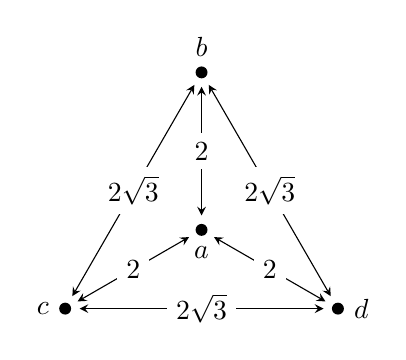
\begin{tikzpicture}[ >=stealth,
      dot/.style={circle,fill=black,inner sep=0,minimum size=1ex},
      len/.style={<->,shorten >=1mm,shorten <=1mm} ]
      % points
      \node[dot,label=below:{$a$}] (a) at (0,0) {};
      \node[dot,label=above:{$b$}] (b) at (90:2) {};
      \node[dot,label=left:{$c$}] (c) at (210:2) {};
      \node[dot,label=right:{$d$}] (d) at (330:2) {};

      % lengths
      \draw [len] (b) to (c);
      \draw [len] (c) to (d);
      \draw [len] (d) to (b);

      \draw [len] (a) to (b);
      \draw [len] (a) to (c);
      \draw [len] (a) to (d);      

      % labels
      \node[fill=white] at (270:1) {$2\sqrt{3}$};
      \node[fill=white] at (30:1) {$2\sqrt{3}$};
      \node[fill=white] at (150:1) {$2\sqrt{3}$};

      \node[fill=white] at (90:1) {$2$};
      \node[fill=white] at (210:1) {$2$};
      \node[fill=white] at (330:1) {$2$};
    \end{tikzpicture}
  \caption{A dataset in Euclidean space consisting of three points arranged in
  an equilateral triangle with another point at the centre.}
  \label{fig:points-in-plane}
\end{figure}

An all-squares optimal clustering, on the other hand, is not necessarily
linearly separable.  This can be shown by a simple example.  Consider a
dataset consisting of distinct points $a,b,c,d$ arranged in the Euclidean
plane as illustrated in Figure~\ref{fig:points-in-plane}.  There are $n$
copies of $a$ and one copy each of $b,c,d$.  The clustering $\clus =
\{\{(a,n)\},\{(b,1),(c,1),(d,1)\}\}$ has an all-squares cost of 72.  But if we
move one of $b,c,d$ into the first cluster, then we have a cost of $8n+24$
which is greater whenever $n>6$.  Similarly if we move two of $b,c,d$ into the
first cluster we get a cost of $16n+24$.  So whenever $n>6$ the all-squares
optimal clustering is $\clus$ and hence is not linearly separable.

% \subsection{Methods for finding optimal clusterings}
% \label{sec:meth-find-optim}

% In this paper we do not present any new methods for computing optimal
% clusterings, but we will briefly discuss existing methods and other
% possibilities here.  Optimal clustering is intuitively a hard problem.
% Centroid-distance clustering in Euclidean space was taken to be NP-complete
% for decades although this was proved only relatively
% recently\citep{aloise09exact}.  In the next section we will see that
% all-squares clustering is also NP-complete and for both problems we
% investigate the complexity for specific, very simple metric spaces.

% The consequence of the complexity of the problems is that heuristic algorithms
% for estimating optimal solutions are very prevalent; indeed, the $k$-means
% heuristic algorithm (also known as Lloyd's algorithm, although it was
% independently discovered by many different authors\citep{jain2010data}) for
% estimating the centroid-distance optimal $k$-clustering is probably the most
% well-known and widely-used clustering algorithm today.  Assuming that
% centroids are easy to compute, this algorithm is simple and, generally,
% quickly converges to a local optimum.  However, in the worst case, $k$-means
% requires exponentially many iterations in order to converge on a solution,
% even in the plane\citep{vattani2009exponential}.  There are many more
% heuristic methods for the problem; nine prominent methods are compared in
% \citep{brusco2007comparison}.

% Some algorithms for exactly solving the centroid-distance problem are known
% including methods using branch-and-bound \citep{brusco2006repetitive},
% branch-and-cut \citep{aloise09exact} and column generation
% \citep{merle1999interior}.  Some of these algorithms are able to exactly solve
% instances in the plane of around 2000 elements in reasonable time
% \citep{aloise09exact}.

% The all-squares problem, or more generally sum-of-cliques, has received less
% attention but there are, nonetheless, a number of algorithms described in the
% literature.  An exact algorithm using branch-and-bound
% \citep{klein1991optimal} can be used to solve problems with $n \leq 50, k \leq
% 5$ \citep{hansen1997mathprog}.  Cutting planes have also been applied with
% problems with $n \leq 158$ solved quickly
% \citep{hansen1997mathprog,palubeckis1997branch}.  In terms of heuristic
% approaches, there is an obvious iterative agglomerative technique that can be
% applied.  We have a simple randomised version that is showing some promise
% \citep{gk2012agglomerative}.
\clearpage
\section{Complexity issues}
\label{sec:complexity-issues}

\textsc{We will now} formally define the problems of finding an optimal
clustering according to either criteria and analyse the complexity of these
problems.

\subsection{All-squares clustering}
\label{sec:all-squar-clust}

We state the all-squares problem formally as a decision problem:
\begin{problem}{All-Squares Clustering (ASC)}
  \instance{A multiset of nodes $(\dset,\mu_{\dset})$, where $\dset =
    \{S_1,S_2,\dotsc,S_n\}$; a metric, $d$, which is defined for all elements
    in $\dset$; the number of clusters desired, $k \in \mathbb{Z}^+$ and a
    bound $B \in \mathbb{R}^+$.}  \question{Is there a $k$-clustering, $\clus
    = \{C_1,C_2,\dotsc,C_k\}$, such that
    \begin{equation*}
      cost_{as}(\clus)=
      \sum_{i=1}^{k} \sum_{x,y \in C_i} \mu_{C_i}(x)\mu_{C_i}(y)d^2(x,y)
      \leq B \quad \text{?}
    \end{equation*}}
\end{problem}

The problem is defined for multisets but, unless stated otherwise, the
NP-completeness proofs which follow are for sets, since this establishes the
result for multisets too.  When dealing with sets, the membership functions
are omitted since they are always equal to 1.

% so the cost function becomes simply
% \begin{equation*}
%   cost_{as}(\clus)=
%   \sum_{i=1}^{k} \sum_{x,y \in C_i} d^2(x,y).
% \end{equation*}

\subsubsection{Euclidean space}
\label{sec:euclidean-space}

An important special case of ASC is when the nodes are in Euclidean space and
we use the Euclidean metric $d_E$.  We call this special case Euclidean
all-squares clustering (EASC).

\begin{thm}
  EASC is NP-complete.
\end{thm}

\begin{proof}
  We observe that a guessed solution, $\clus_g$, can be checked in polynomial
  time by simply calculating $cost_{as}(\clus_g)$ and comparing the value to
  the bound.  Therefore $\text{EASC} \in \NP$.
  
  Now to show that EASC is NP-complete we construct a transformation from a
  known NP-complete problem to our problem.  The NP-complete problem we will
  use is the following \citep{gareyjohnson79}:
  \begin{problem}{Partition into Triangles (PT)}
    \instance{Graph $G = (V,E)$, with $|V| = 3q$ for some integer $q$.}
    \question{Can each of the vertices of $G$ be partitioned into $q$ disjoint
      sets $V_1,V_2,\dotsc,V_q$, each containing exactly $3$ vertices, such
      that for each $V_i = \{u_i,v_i,w_i\}$, $1 \leq i \leq q$, all three of the
      edges $\{u_i,v_i\}, \{u_i,w_i\}$ and $\{v_i,w_i\}$ belong to $E$?}
  \end{problem}

  We transform an instance $I = G = (V,E)$ of PT, where $|V|=3p$, $V = \{v_0,
  \dotsc, v_{3p-1}\}$ and $|E|=m$ into an instance $f(I)$ of EASC: first we
  assign to $\dset$ a set of $n=3p$ points in $(3p+m)$-dimensional Euclidean
  space.  Each element $v_i \in V$ corresponds to a point where
  \begin{enumerate}
  \item the $i$th coordinate is $N = 2m$,
  \item all other coordinates $1 \leq i \leq 3p$ are 0,
  \item for $1 \leq j \leq m$, if $v_i$ is incident with $e_j \in E$ then the
    $(3p+j)$th coordinate is 1, otherwise it is 0.
  \end{enumerate}
  We then set $k$ to $p$ and $B$ to $8m-12p+12N^2p$.  It is easy to see that
  this transformation can be computed in polynomial time.

  \begin{lem}
    \label{lem:eq-dis}
    Let $\dset$ be a dataset with $|\dset| = n$ where the distance squared
    between each pair of distinct elements is $s$.  The sum-of-squares minimal
    $k$-clustering will contain clusters with cardinality of either
    $\left\lceil \frac{n}{k} \right\rceil$ or $\left\lfloor \frac{n}{k}
    \right\rfloor$ only.
  \end{lem}

  \begin{proof}
    The cost associated with a cluster, $C$, which contains $p$ elements is
    $p(p-1)s = (p^2-p)s$.  The extra cost of adding an element to $C$ is
    $((p+1)^2 - (p+1))s - (p^2-p)s = 2ps$, and the saving when removing an
    element is $(p^2 - p)s - ((p-1)^2 - (p-1))s = 2(p - 1)s$.

    We proceed by contradiction.  Assume that we have an optimal
    $k$-clustering, where $k \geq 2$ (the case where $k=1$ is trivial),
    including two clusters $C_i$ and $C_j$, where $|C_i| = p_i$, $|C_j| = p_j$
    and $p_i > p_j + 1$.  We move an element from $C_i$ to $C_j$; the
    difference in overall cost due to the move is $2p_js - 2p_is + 2s < 0$, so
    we have a saving.  Therefore our original clustering could not have been
    optimal.
  \end{proof}

  \begin{cor}
    \label{cor:extra-cost}
    Since $p_i \geq p_j + 2$, the difference in cost will be $(2p_j - 2p_i +
    2)s \leq 2s$.  Therefore, the cost of any suboptimal clustering will be at
    least $2s$ greater than the cost of the optimal clustering.
  \end{cor}

  In our reduction $\left\lceil \frac{n}{k} \right\rceil = \left\lfloor
    \frac{n}{k} \right\rfloor = 3$, so the optimal clustering when all nonzero
  distances are equal will be one where each cluster contains three elements.

  \begin{lem}
    \label{lem:euclidean-iff}
    $I$ is a YES instance of PT if and only if $f(I)$ is a YES instance of EASC.
  \end{lem}

  \begin{proof}
    If $I \in Y_{\text{PT}}$ then we can construct a clustering by letting
    each cluster correspond to one of the triangles in the partition of $G$.
    Let $w,x,y$ be the vertices of such a triangle, and therefore a cluster.
    The distance squared between a pair of these points is $d^2(w,x) =
    2N^2+\deg(w)+\deg(x)-2$; the $2N^2$ comes from the coordinates governed by
    rules 1 and 2 in the transformation and the $\deg(w) + \deg(x) - 2$ comes
    from the coordinates governed by rule 3.  The overall cost of the
    clustering is therefore $2(2\deg(w)+2\deg(x)+2\deg(y)+6N^2-6)$.  Hence,
    the set of $p$ triangles has cost
    \begin{equation}
      \label{eq:tri-cost}
      4\sum_{v \in V} \deg(v) + 12N^2p - 12p = 8m + 12N^2p - 12p = B,
    \end{equation}
    so $f(I) \in Y_{\text{EASC}}$.

    If $f(I) \in Y_{\text{EASC}}$ then we have a $k$-clustering which fits the
    bound.  The distance between each pair of distinct points in the dataset
    is at least $2N^2$.  Assume that the distances are all exactly $2N^2$: due
    to Lemma~\ref{lem:eq-dis}, the optimal clustering in this case is one
    where each cluster contains 3 elements, and this clustering has an overall
    cost of $12N^2p$.  Due to Corollary~\ref{cor:extra-cost}, any suboptimal
    clustering would have an overall cost of at least $(12p+4)N^2$ and, since
    $N^2=4m^2$, will not meet the bound.  Clearly, if one of these suboptimal
    clusterings contained distances greater than $2N^2$ in the sum their
    overall cost would be greater still.  Therefore, each cluster must contain
    exactly 3 elements.

    As shown in equation~\eqref{eq:tri-cost}, the cost of a clustering where
    each cluster corresponds to a triangle in $G$ equals the bound.  If some
    cluster does not correspond to a triangle, then its cost is increased, and
    therefore the overall cost of the clustering will be greater than the
    bound.  So each cluster must be a triangle, so $I \in Y_{\text{PT}}$.
  \end{proof}
  Hence, due to Lemma~\ref{lem:euclidean-iff}, the theorem is established.
\end{proof}

\subsubsection{$p$-valued metric}
\label{sec:p-valued-metric}

\begin{dfn}
  A \textbf{$p$-valued metric} is a metric where the cardinality of the
  codomain is equal to some positive integer $p$.
\end{dfn}

\begin{thm}
  \label{thm:np-complete-3-val}
  ASC is NP-complete even with a 3-valued metric.
\end{thm}

\begin{proof}
  We observe that a guessed solution can be checked in polynomial time,
  therefore $\text{ASC} \in \NP$.

  Now we choose again to construct a transformation from \textsc{Partition
    into Triangles} (PT).  An instance $I$ of PT is transformed into an
  instance $f(I)$ of ASC as follows: first we construct a 3-valued metric
  space by setting $\dset$ to $V$ and defining a function $d \colon \dset
  \times \dset \to \{0,\alpha,\beta\}$ where $0 > \alpha > \beta$ by
  \begin{equation*}
    d(u,v) = \begin{cases}
      0 & \text{if $u=v$,}\\
      \alpha & \text{if there exists an edge in $G$ between $u$ and $v$,}\\
      \beta & \text{otherwise.}
    \end{cases}
  \end{equation*}

  \begin{lem}
    \label{lem:3-val-met}
    $(\dset,d)$ is a metric space.
  \end{lem}
  
  \begin{proof}
    We show that $d$ satisfies each condition required for a metric for all
    $u,v,w \in \dset$:
    \begin{enumerate}
    \item $d(u,v)=0$ if and only if $u=v$ by definition,
    \item $d(u,v)=d(v,u)$ by definition,
    \item $d(u,v)+d(v,w) \geq d(u,w)$ (triangle inequality)\\
      If $u=w$ then this is trivially true.\\
      If $d(u,w)=\alpha$ then $u \neq w$ so either $u \neq v$ or $v \neq w$ or
      both.\\
      If $d(u,w)=\beta$ then $u \neq w$ and there is no edge between $u$ and
      $w$, we then have two cases: either both $u \neq v$ and $v \neq w$ which
      satisfies the inequality, or one of $u=v$ or $v=w$, but we know there is
      no edge between $u$ and $w$ so therefore there is no edge between $v$
      and $w$ or $v$ and $u$ respectively, so the inequality is satisfied.
    \end{enumerate}
  \end{proof}

  We then set $B$ to $6q\alpha$ and $k$ to $q$ to complete the transformation.
  It is easy to see that this transformation can be computed in polynomial
  time.

  \begin{lem}
    \label{lem:3-val-iff}
    $I$ is a YES instance of PT if and only if $f(I)$ is a YES instance of ASC.
  \end{lem}

  \begin{proof}
    If $I \in Y_{\text{PT}}$ then observe that we can construct a clustering,
    $\clus$, by assigning to each cluster $C_i$ the set $V_i$.  Since each
    $V_i$ has an edge between each pair of vertices, the cost of each cluster
    $C_i$ is $6\alpha$, and therefore the cost of $\clus$ is $6q\alpha$.  So
    therefore $f(I) \in Y_{\text{ASC}}$.

    If $I \in N_{\text{PT}}$ then we cannot have a clustering where all
    clusters have cardinality $3$ as this will contain at least one distance
    greater than $\alpha$ and therefore not meet the bound.  We must consider
    clusterings where all within cluster distances are equal to $\alpha$, but
    due to Lemma~\ref{lem:eq-dis}, any such clustering with clusters of
    different sizes always has a higher cost so they also cannot meet the
    bound.  Therefore $f(I) \in N_{\text{ASC}}$.
  \end{proof}

  Hence, due to Lemmata~\ref{lem:3-val-met} and \ref{lem:3-val-iff}, the
  theorem is established.

\end{proof}

\begin{thm}
  \label{thm:asc-np-complete-n-val}
  For all $n \geq 3$ there exists a metric such that ASC is hard, therefore
  ASC is NP-complete with an n-valued metric when $n \geq 3$.
\end{thm}

\begin{proof}
  We proceed by induction.  Theorem~\ref{thm:np-complete-3-val} establishes
  the base case, so we now assume that the problem is NP-complete with an
  $n$-valued metric and show that it is NP-complete with an $(n+1)$-valued
  metric.

  We transform an instance, $I$, of the $n$-valued problem into an instance,
  $f(I)$ of the $(n+1)$-valued problem.  Let $\dset^*$, $d^*$, $k^*$ and $B^*$
  be the dataset, metric, number of clusters and bound of $f(I)$,
  respectively.  We set $\dset^*$ to $\dset \cup \{a\}$, $k^*$ to $k+1$ and
  $B^*$ to $B$.  We define a function $d^* \colon \dset \times \dset$ by
  \begin{equation*}
    d^*(x,y) =
    \begin{cases}
      0 & \text{if $x=y$,}\\
      s & \text{if $x=a$ or $y=a$,}\\
      d(x,y) & \text{otherwise,}
    \end{cases}
  \end{equation*}
  where $s = \sum_{p,q \in \dset} d^2(p,q)$.  Notice that the distance between
  $a$ and each element in $\dset$ is the complete sum of all distances squared
  in $\dset$.  It is easy to see that this transformation can be computed in
  polynomial time.

  \begin{lem}
    \label{lem-asc-n-val-iff}
    $I$ is a YES instance of $n$-valued ASC if and only if $f(I)$ is a YES
    instance of $(n+1)$-valued ASC.
  \end{lem}
  \begin{proof}
    If $I \in Y_{ASC}$ then there is some clustering $\clus =
    \{C_1,C_2,\dotsc,C_k\}$ of $\dset$ with a cost less than or equal to $B$.
    We can construct a similar clustering of $\dset^*$ : $\clus^* = \clus \cup
    \{\{a\}\}$.  The extra cluster will not contribute to the cost, so the
    cost of $\clus^*$ is also less than or equal to $B$, so $f(I) \in
    Y_{ASC}$.

    If $f(I) \in Y_{ASC}$ then there is some clustering, $\clus^* =
    \{C^*_1,C^*_2,\dotsc, C^*_{k^*}\}$, with cost less than or equal to $B$.
    Let $C^*_l$ be the cluster which contains the element $a$.  If some other
    elements belong to this cluster then we can move them into any other
    cluster: each element we move makes a saving of at least $s^2$ but the
    final overall cost of the cluster we move them to can be at worst $s$, so
    clearly this will result in a saving.  Now, $C_l$ contains only $a$ so
    does not contribute to the overall cost, so $\clus^* \setminus C^*_l$ has
    an overall cost less than or equal to $B$ and therefore $I \in Y_{ASC}$.
  \end{proof}

  Hence, due to Lemma~\ref{lem-asc-n-val-iff}, the theorem is established.
\end{proof}

If our dataset is a set and the metric is 2-valued then the problem is
solvable in polynomial time due to Lemma~\ref{lem:eq-dis}.  We need only solve
the equation
\begin{equation*}
  x \left\lceil\frac{n}{k}\right\rceil
  + (k-x) \left\lfloor\frac{n}{k}\right\rfloor = n
\end{equation*}
for $x$ and an optimal clustering is then $x = n-k\lfloor\frac{n}{k}\rfloor$
clusters of $\lceil\frac{n}{k}\rceil$ elements and $k-x$ clusters of
$\lfloor\frac{n}{k}\rfloor$ elements.  For the decision version we would then
simply calculate the cost of the clustering to see if it is less than the
bound.  We conclude with:
\begin{thm}
  When the dataset is a set with a 2-valued metric, an optimal clustering can
  be found in polynomial time.
\end{thm}

However, if the dataset is a multiset this is not the case; the problem
becomes NP-complete.
\begin{thm}
  \label{thm:2-met-multiset-np-complete}
  When the dataset is a multiset with a 2-valued metric, ASC is an NP-complete
  problem.
\end{thm}

\begin{proof}
  We construct a transformation from the NP-complete problem
  \citep{gareyjohnson79}:
  \begin{problem}{Minimum Sum-of-Squares (MSS)}
    \instance{Finite set $A$, a size $s(a) \in \mathbb{Z}^+$ for each $a \in
      A$, positive integers $K \leq |A|$ and $J$.}
    \question{Can $A$ be partitioned into $K$ disjoint sets
      $A_1,A_2,\dotsc,A_k$ such that
      \begin{equation*}
        \sum_{i=1}^{K}\left(\sum_{a \in A_i} s(a)\right)^2 \leq J \quad ?
      \end{equation*}
    }
  \end{problem}
  We construct our dataset by setting $\dset$ to $A$ and $\mu_{\dset}$ to $s$
  and we set $k$ to $K$.  We define a metric $d$ for all $u,v \in \dset$ as
  \begin{equation*}
    d(u,v) =
    \begin{cases}
      0 & \text{if $u=v$,}\\
      1 & \text{otherwise.}
    \end{cases}
  \end{equation*}

  To find the value for $B$, consider an optimal multiset clustering
  $\clus=\{C_1,\dotsc,C_k\}$ which is consistent, so
  $\mu_{C_i}(x)=\mu_{\dset}(x)$ for all $x \in \dset$ and $1 \leq i \leq k$.
  The cost of a single cluster, $C_i$, is
  \begin{equation*}
    \sum_{x,y \in C_i} \mu_{\dset}(x)\mu_{\dset}(y)
    = \left(\sum_{x \in C_i} \mu_{\dset}(x)\right)^2
    - \sum_{x \in C_i} (\mu_{\dset}(x))^2,
  \end{equation*}
  so the total cost of $\clus$ is
  \begin{equation}
    \label{eq:clus-tot}
    \sum_{i=1}^{k}\left(\sum_{x \in C_i} \mu_{\dset}(x)\right)^2
    - \sum_{i=1}^{k}\sum_{x \in C_i} (\mu_{\dset}(x))^2.
  \end{equation}
  The second term is a constant and is equivalent to
  \begin{equation*}
    \Gamma = \sum_{x \in \dset} (\mu_{\dset}(x))^2.
  \end{equation*}
  We set $B$ to $J-\Gamma$ and the transformation is complete.  It is now easy
  to see that the cost of the optimal clustering, $\clus$, will meet the
  bound, $B$, if and only if the first term in expression~\eqref{eq:clus-tot}
  is less than or equal to $J$.  So $I \in Y_{\text{MSS}}$ if and only if
  $f(I) \in Y_{\text{ASC}}$ and the theorem is established.
\end{proof}

\subsection{Centroid-distance clustering}
\label{sec:centr-dist-clust}

Again, we state the problem formally as a decision problem:
\begin{problem}{Centroid-Distance Clustering (CDC)}
  \instance{A metric space $(M,d)$, a set of nodes $\dset \subseteq M$, the
    number of clusters desired, $k \in \mathbb{Z}^+$, and a bound, $B \in
    \mathbb{R}^+$.}
  \question{Is there a $k$-clustering, $\clus = \{C_1,C_2,\dotsc,C_k\}$ such
    that
    \begin{equation*}
      cost_{cd}(\clus)
      = \sum_{i=1}^{k} \sum_{x \in C_i} \mu_i(x) d^2(x,c_i) \leq B,
    \end{equation*}
    where $c_i \in M$ is the centroid of cluster $C_i$?
  }
\end{problem}
Again, the problem is defined for multisets, but the following proof is for
sets so the membership function has been omitted.

\begin{thm}
  \label{thm:CDC-NP}
  CDC is NP-complete.
\end{thm}

\begin{proof}
  We observe that a guessed solution, $\clus_g$, can be checked in polynomial
  time, therefore $\text{CDC} \in \NP$.

  To show that CDC is NP-complete we will construct a transformation from a
  known NP-complete problem to our problem.  The problem we will use is the
  following \cite{gareyjohnson79}:
  \begin{problem}{Dominating Set (DS)}
    \instance{A graph $G=(V,E)$ and a positive integer $K \leq |V|$.}
    \question{Is there a dominating set of size $K$ or less for $G$ or, in
      other words, a subset $V' \subseteq V$ with $|V'| \leq K$ such that for
      all $u \in V \setminus V'$ there is a $v \in V'$ for which $\{u,v\} \in
      E$?  }
  \end{problem}

  We transform an instance $I$ of DS into an instance $f(I)$ of CDC.  Fist we
  construct a 3-valued metric space by setting $M = \dset$ to $V$ and define a
  function $d \colon M \times M \to \rr$ by
  \begin{equation*}
    d(u,v) = \begin{cases}
      0 & \text{if $u=v$,}\\
      1 & \text{if there exists an edge in $G$ between $u$ and $v$,}\\
      2 & \text{otherwise.}
    \end{cases}
  \end{equation*}

  This is a metric space by Lemma~\ref{lem:3-val-met}. We then set $k$ to $K$
  and $B$ to $n-k$.

  \begin{lem}
    \label{lem:iff}
    $I$ is a YES instance of DS if and only if $f(I)$ is a YES instance of CDC.
  \end{lem}

  \begin{proof}
    If $I \in Y_{DS}$ then $|V'| \leq K = k$.  We can construct a
    $k$-clustering by first picking $k-|V'|$ arbitrary elements from $V
    \setminus V'$ and adding each of these to separate clusters.  These are
    final clusters and will not contribute to the overall cost.  We then add
    one element of the dominating set each to the remaining $|V'|$ clusters.
    These elements are the tentative centroids of the clusters.  So far we
    still have an overall cost of zero.  The remaining $n-k$ elements are
    added one by one to any cluster where they share an edge with the
    tentative centroid.  Thus, each of these $n-k$ elements contributes to the
    cost by 1.  If one of the final centroids of these constructed clusters
    turns out to be different to the tentative centroids, this can only
    decrease the cost of that cluster, by the definition of a centroid.
    Therefore the overall cost is less than or equal to $B = n-k$, so $f(I)
    \in Y_{CDC}$.

    \begin{figure}
      \centering
      \begin{tikzpicture}[
        node/.style={circle,fill=black,inner sep=0,minimum size=1ex},
        cent/.style={star,star point height=0.6mm,fill=black,inner sep=0,minimum size=2.5mm},
        edge/.style={-},
        outl/.style={dashed},
        help/.style={inner sep=0,minimum size=0mm}]

        % dominating set nodes (centroids)
        \node[cent] (1) at (0,0) {};
        \node[cent] (2) at (70:1) {};
        \node[cent] (3) at (210:1) {};

        % other nodes
        \begin{scope}
          \node[node] (11) at (0:1) {};
          \node[node] (12) at (135:1) {};
          \node[node] (13) at (270:1) {};
          \node[node] (14) at (315:1) {};
          % helpers
          \node[help] (1h1) at (135:0.2) {};
          \node[help] (1h2) at (-20:0.2) {};
          \node[help] (1h3) at (300:0.2) {};
        \end{scope}
        
        \begin{scope}[shift={(70:1)}]
          \node[node] (21) at (45:1) {};
          \node[node] (22) at (90:1) {};
          % helpers
          \node[help] (2h1) at (-20:0.2) {};
          \node[help] (2h2) at (70:0.2) {};
          \node[help] (2h3) at (160:0.2) {};
        \end{scope}

        \begin{scope}[shift={(210:1)}]
          \node[node] (31) at (225:1) {};
          \node[node] (32) at (180:1) {};
          % helpers
          \node[help] (3h1) at (120:0.2) {};
          \node[help] (3h2) at (210:0.2) {};
          \node[help] (3h3) at (300:0.2) {};
        \end{scope}

        % edges
        \foreach \n in {11,12,13,14} {
          \draw [edge] (1) to (\n);
        }

        \foreach \n in {21,22} {
          \draw [edge] (2) to (\n);
        }

        \foreach \n in {31,32} {
          \draw [edge] (3) to (\n);
        }

        % dominating set outline
        \draw[outl] (1h1) -- (2h3) to [bend left=45] (2h2) to (2h1) -- (1h2)
        to [bend left=25] (1h3) -- (3h3) to [bend left=45] (3h2) to (3h1) -- (1h1);
      \end{tikzpicture}
      \caption{Each of the $k$ clusters correspond to star graphs with the
        centroid at the centre, so there is a dominating set of size $k$ as
        outlined.}
      \label{fig:domset}
    \end{figure}

    If $f(I) \in Y_{\text{CDC}}$ then we have an overall cost of less than or
    equal to $n-k$.  Since $\dset = M$, each cluster must contain an element
    equal to the centroid of that cluster, so there are exactly $k$ elements
    which do not contribute to the overall cost.  Each of the $n-k$ remaining
    elements must contribute to the cost by at least $1$, so therefore must
    contribute by exactly $1$ giving an overall cost of exactly $n-k$.  Each
    cluster therefore corresponds to a star in $G$, as illustrated in
    Figure~\ref{fig:domset}, so $I \in Y_{\text{DS}}$.
  \end{proof}

  Hence, due to Lemmata~\ref{lem:3-val-met} and \ref{lem:iff}, the theorem is
  established.
\end{proof}

Theorem~\ref{thm:CDC-NP} has already been established using Euclidean space.
In fact, the problem has been shown to be NP-hard for both $k=2$ in general
Euclidean space \citep{aloise09} and for general $k$ in only 2 dimensions
\citep{mahajan09}.  If both $k$ and $d$, the number of dimensions, are fixed,
the problem is exactly solvable in $O(n^{dk+1} \log n)$
time\citep{inaba94weightedvoronoi}.

Our proof establishes the following new result:
\begin{cor}
  Even if the metric, $d$, is a 3-valued metric, centroid-distance clustering
  remains an NP-complete problem.
\end{cor}

\begin{thm}
  \label{thm:cdc-np-complete-n-val}
  For all $n \geq 3$ there exists a metric such that CDC is hard, therefore
  CDC is NP-complete with an n-valued metric when $n \geq 3$.
\end{thm}

\begin{proof}
  We proceed by induction.  Theorem~\ref{thm:CDC-NP} establishes the base
  case, so we now assume that the problem is NP-complete with an $n$-valued
  metric and show that it is NP-complete with an $(n+1)$-valued metric.

  We use the same transformation as used for the proof of
  Theorem~\ref{thm:asc-np-complete-n-val}.

  \begin{lem}
    \label{lem-cdc-n-val-iff}
    $I$ is a YES instance of $n$-valued CDC if and only if $f(I)$ is a YES
    instance of $(n+1)$-valued CDC.
  \end{lem}

  \begin{proof}
    If $I \in Y_{CDC}$ then there is some clustering $\clus =
    \{C_1,C_2,\dotsc,C_k\}$ of $\dset$ with a cost less than or equal to $B$.
    We can construct a similar clustering of $\dset^*$: $\clus^* = \clus \cup
    \{\{a\}\}$.  The extra cluster will not contribute to the cost, so the
    cost of $\clus^*$ is also less than or equal to $B$, so $f(I) \in
    Y_{CDC}$.

    If $f(I) \in Y_{CDC}$ then there is some clustering $\clus^* =
    \{C^*_1,C^*_2,\dotsc,C^*_{k^*}\}$ which has cost less than or equal to
    $B$.  Let $C^*_l$ be the cluster which contains element $a$.  If other
    elements belong to this cluster then the cluster will have cost greater
    than or equal to $s^2$.  We can move all other elements to any other
    cluster, say $C^*_p$, which will reduce the cost of $C^*_l$ to 0, but the
    cost of $C^*_p$ must be less than $s$, so we have an overall saving.  Now
    $C^*_l$ does not contribute to the overall cost, so $\clus^* \setminus
    C^*_l$ has an overall cost less than or equal to $B$ and therefore $I \in
    Y_{CDC}$.
  \end{proof}
  Hence, due to Lemma~\ref{lem-cdc-n-val-iff}, the theorem is established.
\end{proof}

However, when the metric is 2-valued, the problem is solvable in polynomial
time, even in the multiset case.  To see this, let our metric be
\begin{equation*}
  d(u,v) =
  \begin{cases}
    0 & \text{if $u=v$,}\\
    s & \text{otherwise.}
  \end{cases}
\end{equation*}

The overall cost of a clustering will be
\begin{equation*}
  \sum_{i=1}^{k} \sum_{\{x \in C_i,x \neq c_i\}} \mu_{i}(x)s^2
\end{equation*}
or, equivalently,
\begin{equation*}
  \sum_{x \in \dset} \mu_{\dset}(x)s^2 - \sum_{i=1}^{k} \mu_{i}(c_i)s^2.
\end{equation*}
The first term is a constant, so the problem is to simply maximise the second
term.  This can be done by ordering the elements of $\dset$ by their
membership count in descending order and selecting the first $k$ elements.  We
move all copies of each of the selected elements to their own cluster; these
will become the centroids.  The remaining elements may then be moved to an
arbitrary cluster as they will all contribute to the cost by $s$ each in any
case.

\section{The assignment metric}
\label{sec:metr-comp-clust}

\textsc{There are many} existing methods for comparing clusterings.  Many do
not provide us with, or do not have established, bounds so are not very useful
for our purposes.  We will look at two metrics which have upper bounds: the
Variation of Information (VI) (see Section~\ref{sec:inform-theor}) and our
assignment metric which we present here.  The assignment metric is based on
set matching like those discussed in Section~\ref{sec:set-matching}, but
allows any metric to be used for comparing the matched sets.

Let $\mathcal{P}_k$ be the set of all possible $k$-clusterings of $\dset$.
We define the assignment metric as a function $\Delta \colon \mathcal{P}_k
\!\times \mathcal{P}_k \to \mathbb{R}$ where
\begin{equation*}
  \Delta(\clus_1, \clus_2) = \min_{\sigma \in S_k} \sum_{i=1}^{k}
  \delta(C_{1i}, C_{2\sigma(i)})
\end{equation*}
for some $\delta \colon (2^{\dset} \setminus \emptyset) \times (2^{\dset}
\setminus \emptyset) \to \mathbb{R}$ and where $S_k$ is the set of all
possible functions $\sigma \colon \{1, \dotsc, k\} \to \{1, \dotsc, k\}$.

\begin{thm}
  The measure $\Delta$ is a metric on $\mathcal{P}_k$ whenever $\delta$ is a
  metric on $(2^{\dset} \setminus \emptyset)$.
\end{thm}

\begin{proof}
  We show that $\Delta$ satisfies all conditions required for a metric:
  \begin{enumerate}
  \item $\Delta(\clus_1, \clus_2) \geq 0$ trivially since
    $\delta(C_{1i}, C_{2j}) \geq 0$ for all $1 \leq i,j \leq k$ since
    $\delta$ is itself a metric,
  \item If $\clus_1 = \clus_2$ then there exists some $\sigma$ for which
    $C_{1i} = C_{2\sigma(i)}$ so $\delta(C_{1i}, C_{2\sigma(i)}) = 0$ for all
    $1 \leq i \leq k$, so $\Delta(\clus_1, \clus_2) = 0$.

    If $\Delta(\clus_1, \clus_2) = 0$ then $\delta(C_{1i},
    C_{2\sigma(i)}) = 0$ and therefore $C_{1i} = C_{2\sigma(i)}$ for
    some $\sigma$ and all $1 \leq i \leq k$, so $\clus_1 = \clus_2$,
  \item $\Delta(\clus_1, \clus_2) = \Delta(\clus_2, \clus_1)$
    trivially since $\delta(C_{1i}, C_{2j}) = \delta(C_{2j}, C_{1i})$
    for all $1 \leq i,j \leq k$,
  \item Let $\Delta(\clus_1, \clus_2) = \sum_{i=1}^{k} \delta(C_{1i},
    C_{2\sigma(i)})$ for
    some $\sigma \in S_k$\\
    and $\Delta(\clus_2, \clus_3) = \sum_{i=1}^{k} \delta(C_{2i},
    C_{\uptau(i)})$ for some $\uptau \in S_k$.
    
    Then,
    \vspace{-1.5em}
    \begin{align*}
      \Delta(\clus_1, \clus_2) + \Delta(\clus_2, \clus_3) &=
      \sum_{i=1}^{k} \delta(C_{1i},
      C_{2\sigma(i)}) + \delta(C_{2\sigma(i)}, C_{3\uptau(\sigma(i))})\\
      &\geq \sum_{i=1}^{k} \delta(C_{1i},
      C_{3\uptau(\sigma(i))})\quad\text{(due to
        triangle inequality of $\delta$)}\\
      &\geq \min_{\sigma \in S_k} \sum_{i=1}^{k} \delta(C_{1i}, C_{3\sigma(i)})\\
      &= \Delta(\clus_1, \clus_3).
    \end{align*}
  \end{enumerate}
  \vspace{-3.5em}
\end{proof}

Possible choices for the $\delta$ metric are the cardinality of the symmetric
difference, $\delta(A,B) = |A \symdif B|$, and the normalised symmetric
difference, also known as the Jaccard distance, $\delta(A,B) = \frac{|A
  \symdif B|}{|A \cup B|}$.  These are well known metrics with the former
being used often in the literature for comparing sets, for example in
\cite{reynolds2006clustering}.  These two metrics extend naturally to
multisets; the multiset version of symmetric difference is
$\delta((A,\mu_A),(B,\mu_B)) = \sum_{x,y \in A \cup B} |\mu_A(x)-\mu_B(y)|$.

Calculating $\Delta$ amounts to calculating the minimum cost matching between
the clusters.  There are $k!$ possible matchings, but the minimum can be found
in $O(k^3)$ time using the Hungarian algorithm \cite{kuhn1955hungarian}.
Since $k! < k^3$ when $k < 6$, it may be more efficient to simply enumerate
all solutions when $k$ is small.

Clusterings with different $k$ can be compared by the addition of the
pseudometric $||\clus_1|-|\clus_2||$ (ie. the absolute difference between the
set cardinalities).  Let $\mathcal{P}$ be the set of all partitions of
$\dset$.  The assignment metric then becomes a function $\Delta \colon
\mathcal{P} \times \mathcal{P} \to \mathbb{R}$ defined as
\begin{equation*}
  \Delta(\clus_1, \clus_2)
  = \min_{\sigma \in S_k} \sum_{i=1}^{k} \delta(C_{1i},C_{2\sigma(i)})
  + \lambda ||\clus_1|-|\clus_2||,
\end{equation*}
where $k = \min(|C_1|,|C_2|)$, $\delta \colon (2^{\dset}\setminus \emptyset)
\times (2^{\dset}\setminus \emptyset) \to \mathbb{R}$ and $\lambda$ is a
positive real number.

This is most sensible when the metric $\delta$ is bounded or normalised and
$\lambda$ is greater than or equal to the upper bound on $\delta$.
Calculation of the metric using the Hungarian algorithm can then be performed
by a simple modification, namely by setting the cost of matching a set to
nothing as $\lambda$ and finding the minimum matching in the same way.

Using a bounded metric does not limit our choice since any metric can be
bounded.  One general formula for bounding a metric by $[0,1]$ is
\begin{equation}
  \label{eq:met-bound}
  \delta_b (A,B) = \frac{\delta(A,B)}{1+\delta(A,B)}.
\end{equation}
Alternatively, it may be possible to normalise the metric, as with the
normalised symmetric difference metric.

This version of the assignment metric is bounded by $\lambda \cdot
\max(|\clus_1|,|\clus_2|)$, and this bound is approached arbitrarily closely
by $\clus_1 = \{\{1,2,\dotsc,n\}\}$. $\clus_2 = \{\{1\},\{2\},\dotsc,\{n\}\}$
in the limit of large $n$ for any metric $\delta$.  Tighter bounds may exist
for specific choices of $\delta$ and fixed $k$ (we prove one in
Section~\ref{sec:upper-bound}).

In Section~\ref{sec:asgn-met-fuzzy-partitions} we show how the assignment
metric can be used to compare fuzzy partitions and in
Section~\ref{sec:lifting-metric-space} we discuss the use of metrics which are
aware of the underlying metric space of a clustering.  In
Section~\ref{sec:worst-case-perf} we use the symmetric difference to prove a
worst case result for our two clustering criteria.

\subsection{Comparing fuzzy partitions}
\label{sec:asgn-met-fuzzy-partitions}

The assignment metric extends easily to fuzzy partitions.  All we need is a
metric on fuzzy sets.  Here we present such a metric which is analogous to the
symmetric difference.

Let $\mathcal{F}_f$ be the set of all fuzzy sets and $\mathcal{F}_c \subset
\mathcal{F}_f$ the set of all crisp sets.  Note that a crisp set is a special
case of a fuzzy set where
\begin{equation*}
  \mu_A(x) =
  \begin{cases}
    1 & \text{if $x \in A$}\\
    0 & \text{if $x \notin A$}
  \end{cases}
\end{equation*}
for all $A \in \mathcal{F}_c$.

We now define a function $\delta_f \colon \mathcal{F}_f \times \mathcal{F}_f
\to \mathbb{R}$ by
\begin{equation*}
  \delta_f(A,B) = \sum_{x \in \mathcal{R}} |\mu(x,A) - \mu(x,B)|.
\end{equation*}

\begin{thm}
  The measure $\delta_f$ is equivalent to the symmetric difference
  $\delta(A,B) = |A \symdif B|$ for all $A,B \in \mathcal{F}_c$.
\end{thm}

\begin{proof}
  For each $x \in \mathcal{R}$:
  \begin{enumerate}
  \item If $x \notin A$ and $x \notin B$ then $\mu(x,A) = \mu(x,B) = 0$ and
    therefore this does not contribute to the sum in $\delta_f(A,B)$,
  \item if $x \in A$ and $x \notin B$ then $\mu(x,A) = 1$ and $\mu(x,B) = 0$
    so $|\mu(x,A) - \mu(x,B)| = |1 - 0| = 1$,
  \item similarly, if $x \notin A$ and $x \in B$ then $|\mu(x,A) - \mu(x,B)|
    = |0 - 1| = 1$,
  \item if $x \in A$ and $x \in B$ then $|\mu(x,A) - \mu(x,B)| = |1 - 1| = 0$
    and therefore also does not contribute to the sum.
  \end{enumerate}
\end{proof}

For fuzzy sets this measure does correspond to $|A \symdif B| = |A \cup B|
- |A \cap B|$ since
\begin{align*}
  \mu(x, A \cup B) &= \max(\mu(x,A), \mu(x,B))\\
  \mu(x, A \cap B) &= \min(\mu(x,A), \mu(x,B))
\end{align*}
so the cardinality $|A \cup B| - |A \cap B|$ is
\begin{align*}
  &\sum_{x \in \mathcal{R}} \big(\max(\mu(x,A),\mu(x,B)) - \min(\mu(x,A),\mu(x,B))\big)\\
  &= \sum_{x \in \mathcal{R}} |\mu(x,A) - \mu(x,B)|.
\end{align*}

\begin{thm}
  $(\mathcal{F}_f, \delta_f)$ is a metric space.
\end{thm}

\begin{proof}~
  
  \begin{enumerate}
  \item $\delta_f(A,B) = 0 \iff A=B$:
    \begin{align*}
      \delta_f(A,B) = 0 &\iff \mu(x,A) = \mu(x,B) \quad \forall x \in
      \mathcal{R}\\
      &\iff A = B,
    \end{align*}
  \item $\delta_f(A,B) = \delta_f(B,A)$ by definition,
  \item $\delta_f(A,B)+\delta_f(B,C) \geq \delta_f(A,C)$ (the triangle
    inequality):
    \begin{align*}
      \delta_f(A,B) + \delta_f(B,C)
      &= \sum_{x \in \mathcal{R}} |\mu(x,A) - \mu(x,B)|
      + \sum_{x \in \mathcal{R}} |\mu(x,B) - \mu(x,C)|\\
      &= \sum_{x \in \mathcal{R}} \big(|\mu(x,A)-\mu(x,B)|
      + |\mu(x,B)-\mu(x,C)|\big)\\
      &\geq \sum_{x \in \mathcal{R}} |\mu(x,A) - \mu(x,C)|\\
      &= \delta_f(A,C)
    \end{align*}
  \end{enumerate}
\end{proof}

There is also a corresponding normalised version of this metric for use with
the second version of the assignment metric:
  \begin{equation*}
    \delta_{f_n}(A,B) = \frac{|A \symdif B|}{|A \cup B|}.
  \end{equation*}

\subsection{Lifting the underlying metric space}
\label{sec:lifting-metric-space}

\begin{figure}
  \centering
  \begin{subfigure}[b]{0.3\textwidth}
    \begin{tikzpicture}
      \begin{axis}[xmin=0,xmax=10,ymin=0,ymax=10,width=1.2\textwidth,tick label style={font=\tiny}]
        \addplot+[only marks,color=blue,mark=o] table {
          2.0 2.0
          1.0 2.0
          2.0 1.0
          0.9 2.3
          2.1 0.7
          1.4 1.3
          2.6 2.8
          2.3 1.2
          3.6 2.1
          4.6 2.4
          3.6 2.5
          3.4 1.2
        };
        \addplot+[only marks,color=red,mark=x] table {
          8.0 2.0
          6.2 2.6
          8.8 3.9
          7.6 2.4
          7.2 3.2
          5.6 2.0
          8.7 2.4
          8.9 1.5
          7.0 2.0
          6.5 1.7
          7.3 1.6
          5.8 1.5
        };
        \addplot+[only marks,color=brown,mark=triangle] table {
          5.0 8.0
          5.5 8.6
          5.7 7.2
          5.2 6.2
          6.8 8.2
          5.2 6.7
          3.8 9.2
          3.7 8.2
          4.3 6.2
          4.9 6.7
          5.0 9.0
          4.5 8.6
        };
      \end{axis}
    \end{tikzpicture}
    \caption{Clustering $\clus_1$.}
    \label{fig:clus1}
  \end{subfigure}
  \begin{subfigure}[b]{0.3\textwidth}
    \begin{tikzpicture}
      \begin{axis}[xmin=0,xmax=10,ymin=0,ymax=10,width=1.2\textwidth,tick label style={font=\tiny}]
        \addplot+[only marks,color=blue,mark=o] table {
          2.0 2.0
          1.0 2.0
          2.0 1.0
          0.9 2.3
          2.1 0.7
          1.4 1.3
          2.6 2.8
          2.3 1.2
          3.6 2.1
          4.6 2.4
          3.6 2.5
          3.4 1.2
          5.2 6.2
          4.3 6.2
          4.9 6.7
          5.2 6.7        
        };
        \addplot+[only marks,color=red,mark=x] table {
          8.0 2.0
          6.2 2.6
          8.8 3.9
          7.6 2.4
          7.2 3.2
          5.6 2.0
          8.7 2.4
          8.9 1.5
          7.0 2.0
          6.5 1.7
          7.3 1.6
          5.8 1.5
        };
        \addplot+[only marks,color=brown,mark=triangle] table {
          5.0 8.0
          5.5 8.6
          5.7 7.2
          6.8 8.2
          3.8 9.2
          3.7 8.2
          5.0 9.0
          4.5 8.6
        };
      \end{axis}
    \end{tikzpicture}
    \caption{Clustering $\clus_2$.}
    \label{fig:clus2}
  \end{subfigure}
  \begin{subfigure}[b]{0.3\textwidth}
    \begin{tikzpicture}
      \begin{axis}[xmin=0,xmax=10,ymin=0,ymax=10,width=1.2\textwidth,tick label style={font=\tiny}]
        \addplot+[only marks,color=blue,mark=o] table {
          2.0 2.0
          1.0 2.0
          2.0 1.0
          0.9 2.3
          2.1 0.7
          1.4 1.3
          2.6 2.8
          2.3 1.2
          3.6 2.1
          4.6 2.4
          3.6 2.5
          3.4 1.2
          
          6.2 2.6
          5.6 2.0
          6.5 1.7
          5.8 1.5
        };
        \addplot+[only marks,color=red,mark=x] table {
          8.0 2.0
          8.8 3.9
          7.6 2.4
          7.2 3.2
          8.7 2.4
          8.9 1.5
          7.0 2.0
          7.3 1.6
        };
        \addplot+[only marks,color=brown,mark=triangle] table {
          5.0 8.0
          5.5 8.6
          5.7 7.2
          5.2 6.2
          6.8 8.2
          5.2 6.7
          3.8 9.2
          3.7 8.2
          4.3 6.2
          4.9 6.7
          5.0 9.0
          4.5 8.6
        };
      \end{axis}
    \end{tikzpicture}
    \caption{Clustering $\clus_3$.}
    \label{fig:clus3}
  \end{subfigure}
  \caption{Three clusterings on the same dataset.}
  \label{fig:three-clusterings}
\end{figure}


Another possibility that the assignment metric gives us is to use a metric
which is aware of the metric space underlying our clustering.  This overcomes
some of the limitations that are present in most comparison methods
\citep{bae2010comparison}.

Figure~\ref{fig:three-clusterings} shows three possible clusterings,
$\clus_1,\clus_2$ and $\clus_3$ on a given dataset.  The elements in this
dataset exist in the Euclidean plane and are shown in their relative positions
on the page.  Imagine that $\clus_1$ represents the standard clustering and
$\clus_2$ and $\clus_3$ are two alternative clusterings.  We would like to
know which of the alternative clusterings is closest to the standard so we
measure the distance between $\clus_1$ and $\clus_2$ and $\clus_1$ and
$\clus_3$.  Under the VI metric we get $\Delta(\clus_1,\clus_2) =
\Delta(\clus_1,\clus_3) = 3.1154556$.  Under the assignment metric with the
symmetric difference we similarly get $\Delta(\clus_1,\clus_2) =
\Delta(\clus_1,\clus_3) = 72$.  This seems contrary to our intuition: we would
expect that $\clus_2$ is further from the standard since the clusters are of
very different shapes.  The assignment metric combined with the Hausdorff
metric $\delta_{H}$ and Euclidean metric $d_E$ reflects this intuition: we get
$\Delta(\clus_1,\clus_2) = 6.0621233$ and $\Delta(\clus_1,\clus_3) =
3.424846$.  We could, of course, have used a metric other than the Euclidean
metric to plug in to the Hausdorff metric if this made more sense.

The Hausdorff metric can be normalised in a natural way for use with the
second version of the assignment metric.  One way would be to divide by the
maximum distance observed in the dataset:
\begin{equation*}
  \delta_{H_n}(X,Y) = \frac{\delta_{H}(X,Y)}{\max_{x,y \in \dset} d(x,y)}.
\end{equation*}

When we use a metric like the Hausdorff metric we have three ``layers'' of
metric space that we are dealing with.  The underlying layer is our dataset
and metric used for clustering $(\dset, d)$.  We have the cluster layer
$(2^{\dset} \setminus \emptyset,\delta)$ and the clustering layer
$(\mathcal{P},\Delta)$.  When we take into account all three layers we say
that we are ``lifting'' the underlying metric space to the space of
partitions.

% Distances between c1 and c2 and c1 and c3 resp.

% VI
% 3.1154556  3.1154556
% asgn met - symdif
% 72
% asgn met - hausdorff
% 6.0621233  3.424846

It should be noted that two commonly used functions for comparing sets in a
metric space
\begin{equation*}
  f_1(X, Y) = \min_{x \in X, y \in Y} d(x, y)
\end{equation*}
and
\begin{equation*}
  f_2(X, Y) = \sum_{x \in X} \sum_{y \in Y} d(x, y)
\end{equation*}
are \textit{not} metrics.  This can be shown by considering a simple
counterexample for each: $f_1(\{x,y\},\{x,z\}) = 0$ violates property 3 of a
metric (identity of indiscernibles) and $f_2(\{x,y\},\{x,y\}) > 0$ violates
property 2 (identical elements are most similar).

\subsection{Upper bound}
\label{sec:upper-bound}

An upper bound for $\Delta$ can be established when $\delta(A,B) = |A \symdif
B|$.  We show the upper bound using sets for clarity, but the result is still
valid for multisets using the multiset version of symmetric difference.

There are $k^2$ possible matchings between clusters, the costs of which can be
shown in a matrix:
\begin{equation*}
  \begin{pmatrix}
    |C_{11} \symdif C_{21}| & |C_{12} \symdif C_{21}|
    & \dots & |C_{1k} \symdif C_{21}| \\
    |C_{11} \symdif C_{22} | & |C_{12} \symdif C_{22} |
    & \dots & |C_{1k} \symdif C_{22} | \\
    \vdots & \vdots & \ddots & \vdots \\
    |C_{11} \symdif C_{2k} | & |C_{12} \symdif C_{2k} |
    & \dots & |C_{1k} \symdif C_{2k} |
  \end{pmatrix}.
\end{equation*}
Let $p_i = |C_{1i}|$, $p_j = |C_{2j}|$ and $p_{ij} = |C_{1i} \cap C_{2j}|$.
We can calculate the sum of the values in the $j$th row of the matrix for some
$j$:
\begin{align*}
  \sum_{i=1}^{k} |C_{1i} \symdif C_{2j}| &= \sum_{i=1}^{k} (|C_{1i} \cup
  C_{2j}| - | C_{1i} \cap C_{2j}|) \\
  &= \sum_{i=1}^{k} (p_j + p_i - 2p_{ij}).
\end{align*}
Noting that $\sum_{i=1}^{k} p_i = m$ and $\sum_{i=1}^{k} p_{ij} = p_j$ this
can be written as
\begin{equation*}
  kp_j + m - 2p_j = (k-2)p_j + m.
\end{equation*}
The total sum of values in the matrix is therefore
\begin{equation*}
  \sum_{j=1}^{k} ((k-2)p_j + m),
\end{equation*}
and noting that $\sum_{j=1}^{k} p_j = m$ we get
\begin{equation*}
  (k-2)m + mk.
\end{equation*}

There are $k!$ possible solutions to the assignment problem where each
solution is a combination of $k$ assignments.  Let $S = \{s_1, s_2, \dotsc,
s_{k!}\}$ be the set of costs for each solution so each element is equal to
$\sum_{i=1}^{k} \delta(C_{1i}, C_{2\sigma(i)})$ for some $\sigma$.  The mean
value in the matrix is
\begin{equation*}
  \frac{(k-2)m + mk}{k^2},
\end{equation*}
so the mean solution value is
\begin{align*}
  \bar{s} &= k \left( \frac{(k-2)m + mk}{k^2} \right)\\
          &= 2m - \frac{2m}{k}.
\end{align*}

We can split $S$ into three disjoint subsets $S_{<}$, $S_{=}$ and $S_{>}$
which contain the solutions which are less than, equal to and greater than the
mean, respectively.  We have two cases: either both $S_{<} = \emptyset$ and
$S_{>} = \emptyset$ or both $S_{<} \neq \emptyset$ and $S_{>} \neq \emptyset$.
In the first case, all solutions are equal to the mean and therefore any of
these will be picked; in the second case, a solution from $S_{<}$ will be
picked.

\begin{figure}
  \centering
  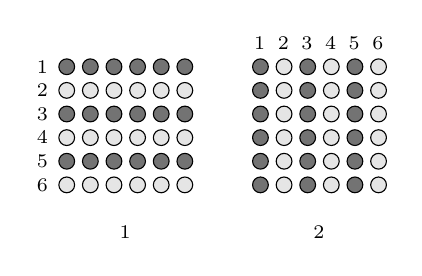
\begin{tikzpicture}[
    poi/.style={circle,draw=black,inner sep=0,minimum size=2mm}
    ]

    % clustering one
    \foreach \y in {0,0.6,1.2} {
      \foreach \x in {0,0.3,0.6,0.9,1.2,1.5} {
        \node[poi,fill=gray!110] at (\x,\y+0.3) {};
        \node[poi,fill=gray!20] at (\x,\y) {};
      }
    }
    % cluster labels
    \foreach \y/\n in {1.5/1,1.2/2,0.9/3,0.6/4,0.3/5,0/6} {
      \node at (-0.3,\y) {$_\n$};
    }

    % clustering label
    \node at (0.75,-0.6) {$\clus_1$};

    % clustering two
    \begin{scope}[xshift=70]
      \foreach \y in {0,0.3,0.6,0.9,1.2,1.5} {
        \foreach \x in {0,0.6,1.2} {
          \node[poi,fill=gray!20] at (\x+0.3,\y) {};
          \node[poi,fill=gray!110] at (\x,\y) {};
        }
      }

      % cluster labels
      \foreach \x/\n in {1.5/6,1.2/5,0.9/4,0.6/3,0.3/2,0/1} {
        \node at (\x,1.8) {$_\n$};
      }

      % clustering label
      \node at (0.75,-0.6) {$\clus_2$};
    \end{scope}

  \end{tikzpicture}
  \caption{Two clusterings, $\clus_1$ and $\clus_2$, formed of six
    clusters each.  These clusterings are optimally different under both the
    assignment metric and variation of information.}
  \label{fig:worst-case}
\end{figure}

Therefore
\begin{equation*}
  \Delta(\clus_1,\clus_2) \leq 2m - \left\lceil \frac{2m}{k} \right\rceil.
\end{equation*}
This bound is tight and can be met with the worst case
\begin{align*}
  \clus_1 = \{&\{1,\dotsc,k\},\{k+1,\dotsc,2k\},\dotsc,\{(k-1)k+1,\dotsc,k^2\}\} \\
  \clus_2 = \{&\{1,k+1,\dotsc,(k-1)k+1\},\\
  &\{2,k+2,\dotsc,(k-1)k+2\},\\
  &\dotsc,\\
  &\{k,k+k,\dotsc,(k-1)k+k\}\}
\end{align*}
which is also shown in Figure~\ref{fig:worst-case}.  This also produces the
worst case under the VI metric, as shown in \citep{meila-2007}.

\section{Worst case performance}
\label{sec:worst-case-perf}

\textsc{We have so far seen} that our two clustering criteria have a number of
similarities, and a number of differences.  Using our metrics for comparing
clusterings, we will now show just how different an all-squares optimal
clustering and a centroid-distance optimal clustering of the same dataset can
be.

\begin{figure}
  \centering
  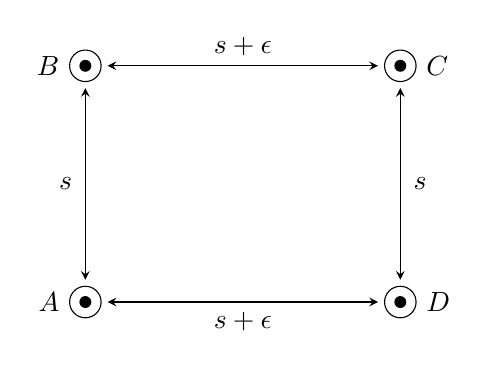
\begin{tikzpicture}[
    >=stealth,
    dot/.style={circle,fill=black,inner sep=0,minimum size=1ex},
    sur/.style={circle,fill=white,draw=black,inner sep=0,minimum size=4mm},
    len/.style={<->,shorten >=2mm,shorten <=2mm}
    ]
    % surrounds
    \node[sur,label=left:{$A$}] (A) at (0,0) {};
    \node[sur,label=left:{$B$}] (B) at (0,3) {};
    \node[sur,label=right:{$C$}] (C) at (4,3) {};
    \node[sur,label=right:{$D$}] (D) at (4,0) {};

    % dots
    \node[dot] (A) at (0,0) {};
    \node[dot] (B) at (0,3) {};
    \node[dot] (C) at (4,0) {};
    \node[dot] (D) at (4,3) {};

    % length arrows
    \draw [len] (A) to (B);
    \draw [len] (B) to (D);
    \draw [len] (D) to (C);
    \draw [len] (C) to (A);

    % length labels
    \node at (-0.25,1.5) {$s$};
    \node at (4.25,1.5) {$s$};

    \node at (2,-0.25) {$s+\epsilon$};
    \node at (2,3.25) {$s+\epsilon$};
  \end{tikzpicture}
  \caption{Relative positions of elements to be clustered.  $A$ and $B$
    contain $N$ elements each, $C$ and $D$ contain $N+1$ elements each.}
  \label{fig:clusters}
\end{figure}

Let $(M,d_E)$ be 2-dimensional Euclidean space with the Euclidean metric and
our dataset be $(\dset, \mu_{\dset})$ where $\dset \subset \mathbb{R}^2$,
$\dset = A \cup B \cup C \cup D$, $\mu_{\dset}(A)=\mu_{\dset}(B)=N$ and
$\mu_{\dset}(C)=\mu_{\dset}(D)=N+1$.  The relative positions of $A,B,C,D$ in
the Euclidean plane are shown in Figure~\ref{fig:clusters}.  Two possible
$2$-clusterings of $(\dset,\mu_{\dset})$ are $\{A \cup B,C \cup D\}$ and $\{A
\cup D,B \cup C\}$ which we will call $\clus_1$ and $\clus_2$ respectively.

Formulae for the all-squares and centroid-distance costs of $\clus_1$ and
$\clus_2$ can now be given, first for centroid-distance cost:
\begin{eqnarray*}
  cost_{cd}(\clus_1) &=& \frac{1}{2}\left(Ns^2+(N+1)s^2\right), \\
  cost_{cd}(\clus_2) &=& \frac{1}{2}\left(N(s+\epsilon)^2+(N+1)(s+\epsilon)^2\right).
\end{eqnarray*}
It is clear that $\clus_1$ is the optimal clustering under the
centroid-distance criterion whenever $\epsilon > 0$.  Now, for all-squares
cost,
\begin{eqnarray*}
  cost_{as}(\clus_1) &=& 2N^2s^2+2(N+1)^2s^2, \\
  cost_{as}(\clus_2) &=& 4N(N+1)(s+\epsilon)^2.
\end{eqnarray*}
So $\clus_2$ is the optimal clustering under the all-squares criterion
whenever
\begin{equation*}
  \epsilon < \sqrt{s^2 + \frac{s^2}{2N(N+1)}} - s.
\end{equation*}
Other clusterings of $\dset$ are possible, but these are trivially more
expensive.

A simple numerical example can now be constructed; let $s=1.4$, $\epsilon=0.1$
and $N=1$.  The costs of all possible 2-clusterings are shown in
Table~\ref{tab:costs}.  Again we see that the optimal clustering under each
criterion is different.

% \begin{table}
%   \centering
%   \caption{The costs of possible 2-clusterings
%     of $\dset$, with minimum costs underlined.}
%   \begin{tabular}{lrr}
%   \toprule
%   Clustering & Centroid-distance cost & All-squares cost \\
%   \midrule
%   $\{A \cup B, C \cup D\}$ & \underline{2.94} & 19.6 \\
%   $\{A \cup D, B \cup C\}$ & 3 & \underline{18} \\
%   $\{A \cup C, B \cup D\}$ & $5\frac{46}{75}$ & 33.68 \\
%   $\{A, B \cup C \cup D\}$ & 4.152 & 41.52 \\
%   $\{C, A \cup B \cup D\}$ & 4.2825 & 29.76 \\
%   \bottomrule
% \end{tabular}
% \label{tab:costs}
% \end{table}

\begin{table}
  \centering
  \caption{The costs of possible 2-clusterings
    of $\dset$, with minimum costs underlined.}
  \begin{tabular}{lrr}
  \toprule
  Clustering & Centroid-distance cost & All-squares cost \\
  \midrule
  $\{A \cup B, C \cup D\}$ & \underline{2.940} & 19.60 \\
  $\{A \cup D, B \cup C\}$ & 3.375 & \underline{18.00} \\
  $\{A \cup C, B \cup D\}$ & 5.613 & 33.68 \\
  $\{A, B \cup C \cup D\}$ & 4.152 & 41.52 \\
  $\{B, A \cup C \cup D\}$ & 4.152 & 41.52 \\
  $\{C, A \cup B \cup D\}$ & 4.283 & 29.76 \\
  $\{D, A \cup B \cup C\}$ & 4.283 & 29.76 \\
  \bottomrule
\end{tabular}
\label{tab:costs}
\end{table}


$\clus_1$ and $\clus_2$ are not just slightly different clusterings, they are
in fact optimally different, that is, no two clusterings can be more
different, according to both the VI metric and assignment metric, as well as
our basic intuition.  This leads us to:
\begin{thm}
  \label{thm:worst-case}
  A centroid-distance optimal clustering and an all-squares optimal clustering
  can be optimally different under both the VI metric and the assignment
  metric.
\end{thm}

\section{Conclusion}
\label{sec:conclusion-sumsq}

\textsc{In this chapter} we have shown that the two sum-of-squares criteria,
centroid-distance and all-squares, share some similarities but also some
differences.  Optimal clusterings according to both criteria may be consistent
but, while centroid-distance always produces linearly separable solutions,
all-squares does not.

Both criteria simultaneously measure both homogeneity and separation.  For
all-squares, the relationship between the homogeneity measure and separation
measure is trivial and independent of the choice of metric.  However, for
centroid-distance we have shown that the homogeneity measure is not
necessarily equivalent to the separation measure when using something other
than the Euclidean metric.  The example we used is the homogeneous
Euclidean-overlap metric for mixed data.

It has recently been shown that the centroid-distance problem is NP-hard using
Euclidean space.  We have shown that both problems are NP-complete even when
using a simple 3-valued metric.  We also show that all-squares is NP-complete
in Euclidean space.  When using a 2-valued metric, both problems are in P,
except for all-squares on a multiset, which remains NP-complete.

We have introduced a new metric for comparing clusterings, called the
assignment metric.  It is, in fact, a family of metrics since any metric for
comparing matched sets can be used.  This allows for some interesting choices
of metric, namely we can use it to compare fuzzy clusterings and take into
account the underlying metric space of the dataset which gives the measure a
more intuitive feel.  We have used this metric to show just how different
optimal clusterings according to the two criteria can be.  It turns out that
they can be optimally different, according to both our metric and the VI
metric.

Much of the work here which we present for multisets also applies naturally to
fuzzy multisets.  The consistency results also extend to crispness, that is to
say that optimal fuzzy clusterings according to either criteria need not have
been fuzzy in the first place.  The assignment metric also applies to fuzzy
clusterings simply by using a metric for fuzzy sets.

% Further work will be done on methods for approximating the optimal clustering
% according to all-squares.  Further applications for the assignment metric and
% new bounds will also be investigated.



%%% Local Variables:
%%% TeX-master: "thesis"
%%% End:
